%%----------------------------------------------------------------------
\section{MASS Planning Module}
\label{s:MASS Planning Module}
%% - - - - - - - - - - - - - - - - - - - - - - - - - - - - - - - - - - -

In this section, we give an overview on the two frameworks for parameter-space exploration, OACIS and CARAVAN.
Although both of these frameworks are designed in order to conduct parameter-space exploration making full use of HPC resources, they differ in the target scale of each job.
In one hand, a certain class of research issues requires to use the maximum computing power to solve a single large problem, so called capability computing.
On the other hand, other researches require to do many small- or medium-scale simulations for parameter-space explorations, i.e., capacity computing.
We categorized these problems into four classes depending on the scale of a single simulation job as summarized in Table~\ref{tab:problem_scale}.
In this Table, it is assumed that the total amount of computation is order of ten exa floating-point operations.
The left most column, which we call class A, corresponds to typical capability computing. The number of independent jobs is at most $10^2$.
In class B, a typical single job is an MPI-parallel program using $10^3 \sim 10^5$ CPU cores. The number of jobs amounts to $10^3 \sim 10^5$.
In this class, a naive manual management of jobs is no longer possible and a framework for managing jobs is necessary.
When typical job scale is serial or shared-memory parallel application, as labelled class C, the number of jobs expands up to $10^6 \sim 10^9$, which requires an even harder job management.
In this class, the parameter selection and interpretation of the results for each job must be done algorithmically.
Finally, on the right most class, where a single job becomes a function level, the number of jobs is more than $10^{10}$.
Thus, for capacity computing ranging from class B to D, the demands for frameworks can be totally different depending on the granularity of jobs.
This is why we developed two frameworks, OACIS and CARAVAN for classes B and C, where majority of the social simulations are found.

\begin{table}[htb]
  \caption{Categorization of the problems according to the scale of single simulation job.
  To calculate the required number of operations, FLOPS, the number of CPU cores for each job, we made assumptions that an exa-flops computer is available, the efficiency of each job is 10\%, and the duration of each job is order of $10^2$ seconds.
  From left to right, the typical scale becomes finer while the typical number of jobs gets greater.
  In the last two lines, we showed an example of social simulations and a framework used for parallel job execution.
  }
  \label{tab:problem_scale}
  \centering
  \begin{tabular}{|c|cccc|} \hline
    class      & A                & B                & C                & D \\ \hline
    \# of jobs & $10^0 \sim 10^2$ & $10^3 \sim 10^5$ & $10^6 \sim 10^9$ & $10^{10} \sim$ \\
    \# of operations / job & $10^{19} \sim 10^{17}$ & $10^{16} \sim 10^{14}$ & $10^{13} \sim 10^{10}$ & $10^{9} \sim$ \\
    FLOPS / job & $10^{18} \sim 10^{16}$ & $10^{15} \sim 10^{13}$ & $10^{12} \sim 10^{9}$ & $10^{8} \sim$ \\
    \# of cores / job & $10^{8} \sim 10^{6}$ & $10^{5} \sim 10^{3}$ & $10^{2} \sim 10^{-1}$ & $10^{-2} \sim$ \\
    typical job scale & large-scale MPI & medium scale MPI & SMP or serial & function \\
    parameter selection & manual & manual or auto & auto & auto \\
    social simulation application & - & traffic in metropolitan area & traffic in a city & data-driven model \\
    frameworks & & OACIS & CARAVAN & Map-Reduce \\
    \hline
  \end{tabular}
\end{table}

OACIS, which stands for Organizing Assistant for Comprehensive and Interactive Simulations, is a job management framework for problems in class B\cite{murase_phys_proc}.
It is available as an open-source software under the MIT license. (http://github.com/crest-cassia/oacis).
This class of problems require researchers to carry out many simulation jobs changing models and parameters by trial and error.
This kind of trial-and-error approach often causes a problem of job management because of a large amount of repetitive works.
Such repetitions are not only troublesome and tedious but prone to human errors.
OACIS is designed to let researchers conduct their research in an efficient, reliable, and reproducible way, helping management of simulation jobs and results.

\begin{figure}
  \centering
  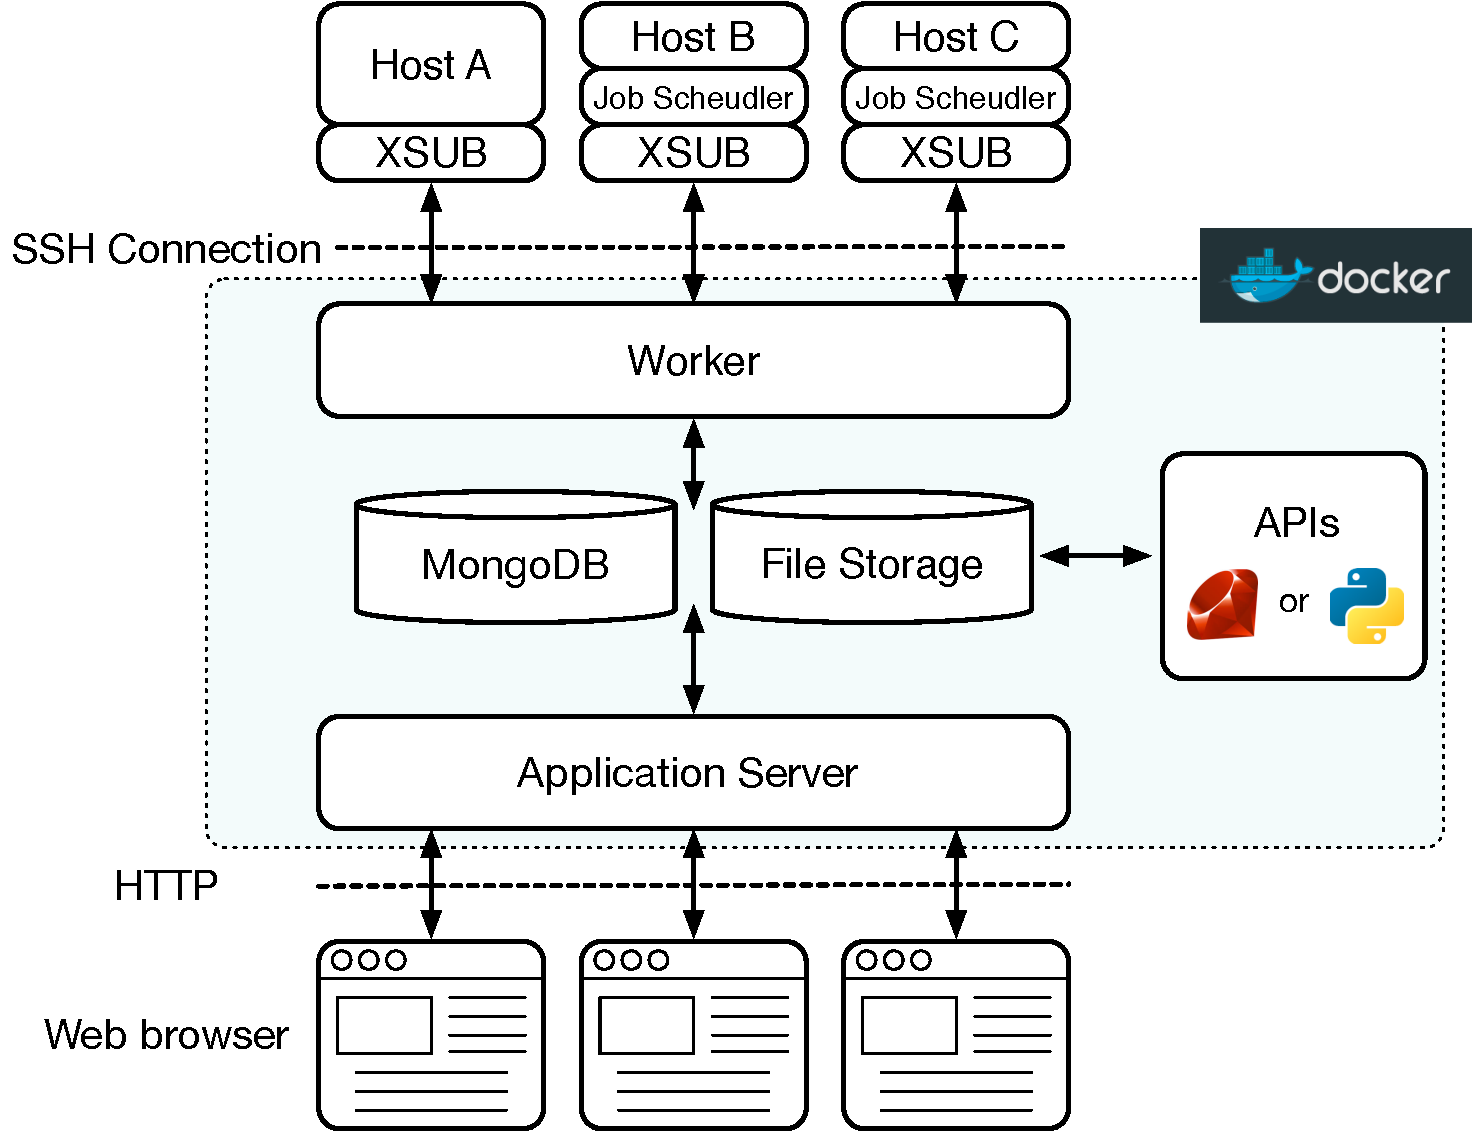
\includegraphics[width=.8\linewidth]{Figs.murase/oacis_overview.pdf}
  \caption{A system overview of OACIS.}
  \label{fig:oacis_overview}
\end{figure}

The system architecture of OACIS is depicted in Fig.~\ref{fig:oacis_overview}.
It is a web application developed based on the Ruby on Rails framework, which provides an interactive user-interface.
The application server is responsible for handling requests from users. When a user creates a job using a web browser, the record of the job is created in the database.
Another daemon process, which we denote as ``worker'', periodically checks whether a job is ready to be submitted to a remote host.
If a job is found, the worker generates a shell script to execute a job and submits it to the job scheduler on the remote host (which we call ``computational hosts'') by SSH connection.
The worker process then periodically checks the status of the submitted jobs and, when the jobs are finished, it downloads the results and stores them into designated storage and database appropriately.
Hence, users do not have to check the job status by themselves and the simulation results are kept in an organized and traceable way.
Various logs, including the values of parameters, executed dates, elapsed times, the version number of the simulator, are automatically kept as well.
A simulator on OACIS is registered as a command line string to execute the simulation, not as the execution program itself.
By this design, OACIS can run simulators in various research fields, which may be written in different programming language.

In addition to an interactive user-interface, OACIS provides application programming interfaces (APIs) in Ruby and Python programming languages.
Any set of operations on OACIS is programmable using the APIs, which can be used for various types of parameter-space explorations including parameter sweeps, sensitivity analysis, and optimization of parameters.

CARAVAN is another framework designed for class C jobs.
It is also available as an open-source software under the MIT license.(https://github.com/crest-cassia/caravan)

Figure~\ref{fig:caravan_overview} shows the whole architecture of CARAVAN. It consists of three parts: search engine, scheduler, and simulator.
``Simulator'' is an executable program prepared for each use case. Once a user integrate a simulator into CARAVAN, it is executed in parallel.
Since a simulator is executed as an external process, a simulator may be implemented in any language as in OACIS.
``Scheduler'' is a part which is responsible for parallelization. It receives the commands to execute simulators from the search engine, distributes them to available nodes, and executes the simulator in parallel.
This part is implemented in X10 programming language using MPI for a communication layer.
``Search engine'' is a part which determines the policy on how parameter-space is explored.
More specifically, it generates a series of commands to be executed in parallel, send them to scheduler.
It also receives the results from the scheduler when these tasks are done.
Based on the received results, search engine can generate other sets of tasks repeatedly as many as a user wants.
This part is written in Python.
A simulator and a search engine must be prepared by each user while the scheduler does not have to be modified once it is built.

When writing a simulator and a search engine, users do not have to explicitly take care of the parallelization.
The scheduler is designed so that the whole application can scale up to tens of thousands of processes.
To evaluate the performance of the scheduler on the K computer, we tested an embarrassingly parallel problem, in which each task takes about 20 seconds.
We obtained a result that the efficiency of the task scheduling remains more than 99\% even when the number of MPI processes is scaled up to 18432.

%%++++++++++++++++++++++++++++++++++++++++++++++++++++++++++++++++++++++
\begin{figure}
  \centering
  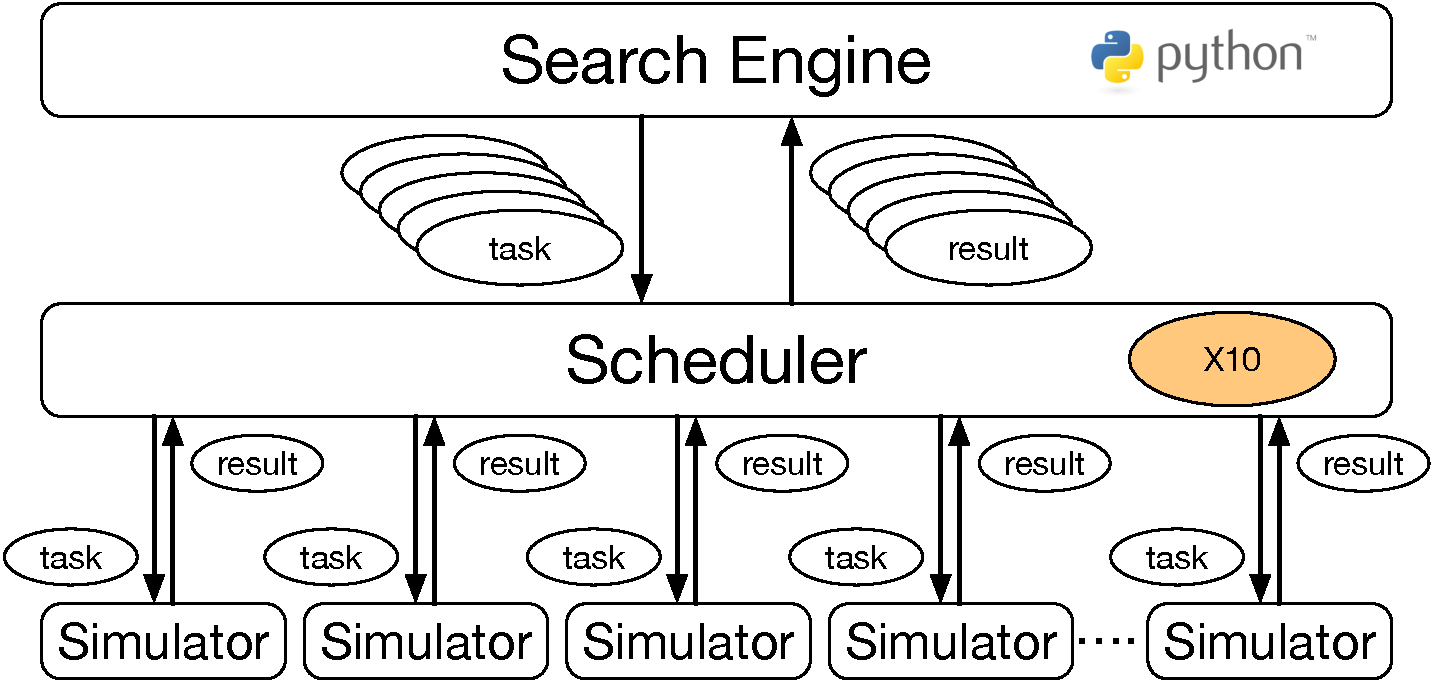
\includegraphics[width=.8\linewidth]{Figs.murase/caravan_overview.pdf}
  \caption{A system overview of CARAVAN}
  \label{fig:caravan_overview}
\end{figure}
%%++++++++++++++++++++++++++++++++++++++++++++++++++++++++++++++++++++++

